
\documentclass{article}

\usepackage{times}
\usepackage{graphicx} % more modern
\usepackage{subfigure} 
\usepackage{natbib}
\usepackage{algorithm, algorithmic}
\usepackage{hyperref}
\newcommand{\theHalgorithm}{\arabic{algorithm}}
\usepackage{amssymb, mathtools}
\usepackage{xcolor,colortbl}




% Employ this version of the ``usepackage'' statement after the paper has
% been accepted, when creating the final version.  This will set the
% note in the first column to ``Proceedings of the...''
\usepackage[accepted]{icml2017}


% The \icmltitle you define below is probably too long as a header.
% Therefore, a short form for the running title is supplied here:
\icmltitlerunning{Globally Induced Forest}

% ============================== PATHS =================================== %
\graphicspath{{./images/}}
% ============================== COLORS =================================== %
\definecolor{orange}{HTML}{FFA500}
\definecolor{dodgerblue}{HTML}{1E90FF}
\definecolor{deepgreen}{HTML}{0AF191}
\definecolor{purplish}{HTML}{E21173}

% ============================== COMMANDS =================================== %
\DeclareMathOperator*{\argmin}{arg\,min}
\DeclareMathOperator*{\argmax}{arg\,max}

\newcommand\pgnote[1]{\textcolor{blue}{\textit{PG: #1}}}

\newcommand{\best}{\cellcolor{lightgray}}
\newcommand{\bestA}{\cellcolor{orange}}
\newcommand{\bestB}{\cellcolor{dodgerblue}}


\begin{document} 
\twocolumn[
\icmltitle{Globally Induced Forest: A Prepruning Compression Scheme}

% It is OKAY to include author information, even for blind
% submissions: the style file will automatically remove it for you
% unless you've provided the [accepted] option to the icml2017
% package.

% list of affiliations. the first argument should be a (short)
% identifier you will use later to specify author affiliations
% Academic affiliations should list Department, University, City, Region, 
%Country
% Industry affiliations should list Company, City, Region, Country

% you can specify symbols, otherwise they are numbered in order
% ideally, you should not use this facility. affiliations will be numbered
% in order of appearance and this is the preferred way.
\icmlsetsymbol{equal}{*}

\begin{icmlauthorlist}
\icmlauthor{Jean-Michel Begon}{ulg}
\icmlauthor{Arnaud Joly}{ulg}
\icmlauthor{Pierre Geurts}{ulg}
\end{icmlauthorlist}

\icmlaffiliation{ulg}{Department of Electrical Engineering and Computer Science
University of Li\`ege, Li\`ege, Belgium}

\icmlcorrespondingauthor{Jean-Michel Begon}{jm.begon@ulg.ac.be}
%\icmlcorrespondingauthor{Arnaud Joly}{a.joly@ulg.ac.be}
\icmlcorrespondingauthor{Pierre Geurts}{p.geurts@ulg.ac.be}

% You may provide any keywords that you 
% find helpful for describing your paper; these are used to populate 
% the "keywords" metadata in the PDF but will not be shown in the document

\icmlkeywords{Decision tree, Random forest, Extremely randomized trees, 
pruning, node budget, memory constraint, compression, growing algorithm, greedy 
selection}

\vskip 0.3in
]

\printAffiliationsAndNotice{}

\begin{abstract} 
Tree-based ensemble models are heavy memory-wise. An undesired state of affairs
considering nowadays datasets, memory-constrained environment and
fitting/prediction times.  In this paper, we propose the Globally Induced Forest
(GIF) to remedy this problem. GIF is a fast prepruning approach to build
lightweight ensembles by iteratively deepening the current forest. It mixes
local and global optimizations to produce accurate predictions under memory
constraints in reasonable time.  We show that the proposed method is more than
competitive with standard tree-based ensembles under corresponding constraints,
and can sometimes even surpass much larger models.
\end{abstract} 

\section{Introduction}
\label{sec:introduction}

Decision forests, such as Random Forest \cite{breiman2001random} and
Extremely Randomized Trees \cite{extratrees}, are popular methods in
the machine learning community. This popularity is due to their
overall good accuracy, relative ease-of-use, short learning/prediction
time and interpretability. However, datasets have become bigger and
bigger over the past decade. The number of instances $N$ has increased
and the community has turned to very high-dimensional learning
problems. The former has led to bigger trees, as the number of nodes
in a tree is $O(N)$. The latter, on the other hand, tends to steer
toward larger forests. Indeed, the variance of individual trees tends
to increase with the dimensionality $P$ of the problem
\cite{l1basedcomp}.  Therefore, the adequate number of trees $T$
increases with the dimensionality.  Overall, this change of focus
might render tree-based ensemble techniques impractical memory-wise,
as the total footprint is $O(N \times T(P))$.

Aside from big data, other areas of machine learning suffer from the
high memory demand of tree-based methods. For instance, low-memory
devices, such as mobile phones and embedded systems, require
lightweight models. %% In addition, bigger is not always better when it
%% comes to tree-based ensembles.  If it is true that the more trees, the
%% better the model, this is not the case for deeper individual trees.
Smaller models also implies faster predictions, which is crucial for real-time
applications. All in all, tree-based models might benefit from lighter memory
footprint in many different ways.

%\vspace*{-\baselineskip}

%\paragraph{Contribution and outline.}
In this paper, we propose the Globally Induced Forest (GIF), an algorithm
which, under a node budget constraint, iteratively and greedily deepens
multiple trees by optimizing {\bf globally} the sequence of nodes to develop
and their associated weights, while still choosing {\bf locally}, based on the
standard local score criterion, the splitting variables and cut points at all
tree nodes.

As a pre-pruning approach, GIFs circumvent the  need to build the whole forest 
first, thus discarding the need for a large temporary storage. This, in 
addition to the mix of global, local and greedy optimization, results in a fast 
method, able to produce lightweight, yet accurate forests learned on the whole 
training set.

After a discussion of the related work in Section \ref{sec:relatedWork},
Section \ref{sec:gif} introduces the GIF algorithm and how it can be applied
for both regression (Section \ref{subsec:regression}) and classification
(Section \ref{subsec:classification}).  In Section \ref{sec:analysis}, we show
that our proposed algorithm, with its default setting, performs well on many
datasets, sometimes even surpassing much larger models. We then conduct an
extensive analysis of its hyper-parameters (Section
\ref{subsec:hyperparams}). Since GIF shares some resemblance to Boosting, the
two approaches are compared in Section \ref{subsec:boosting}, before concluding
and outlining future works in Section \ref{sec:conclusion}.


\section{Related work}
\label{sec:relatedWork}
Memory constraints of tree-based ensemble methods is not a new topic and has
been tackled from various perspectives, which can be partitioned into
tree-agnostic and tree-aware methods. The former set of techniques are general
purpose methods which can deal with any ensembles. We can distinguish further
between re-learning algorithms
\citep[e.g.][]{domingos1997oracle,menke2009oracle}, which try to come up with a
smaller, equivalent models, and ensemble pruning methods. These latter methods
try to eliminate some of the redundant base models constituting the ensemble
but do not attempt to reduce the complexity of the individual models
\citep{tsoumakas2008enspruning,rokach2016enspruning}.
%Why don't we compare to them?

Tree-aware methods strive to build smaller trees by limiting the total number
of nodes within the forest. Several families have been proposed. For instance,
\citet{breiman1999pasting} learns the forest with a subsample of the training
data. Some authors have proposed to relax the trees into DAGs {\it a
  posteriori} at first \citep[e.g.,][]{peterson2009dag} and more recently {\it
  a priori} \cite{shotton2013jungle}.  Similarly, techniques working on the
whole dataset and yielding ensemble of trees can be partitioned into pre- and
post-pruning methods. Pre-pruning methods aim at stopping the development of
uninteresting branches in the top down induction procedure. On the other hand,
the goal of post-pruning methods is to discard {\it a posteriori} subtrees which
do not provide significant accuracy improvements.

Originally, pruning methods were introduced to control the model complexity and
avoid overfitting. The advent of ensemble methods somewhat cast aside those
techniques as the averaging mechanism became responsible for reducing the
variance and rendered pruning mostly unnecessary from the point of view of
accuracy. Nonetheless, a few ensemble-wise, post-pruning methods have recently
emerged with a focus on memory minimization. In both
\cite{meinshausen2009forestgarrote} and \cite{l1basedcomp}, the compression is
formulated as a slightly different global constrained optimization problem.  In
\cite{ren2015glorefinement}, compression is undertook with a sequential
optimization approach by removing iteratively the least interesting leaves.  In
\cite{vleeschouwer2015mitimemreq}, the authors alleviate the leaves' memory
requirements by clustering their conditional distributions. After computing a
wavelet coefficient for each node, \citet{elisha2016wavelet} discard all the
nodes which are not on the path to a node of sufficient coefficient.  All these
methods are able to retain almost the full forest accuracies while offering a
significant memory improvement, leaving their requirement for building the whole
forest first, and consequently the high temporary memory and computational
costs, as their only major drawbacks.

Although our aim is to pre-prune random forests, the GIF algorithm shares
similarity with Boosting methods \cite{friedman2001gradboost}, which fit
additive tree ensembles based on a global criterion and are also able to build
accurate yet small models. Whereas most Boosting methods only explore ensembles
of fixed-size trees, GIF does not put any prior complexity constraint
on the individual trees but instead adapts their shape greedily. It shares this
property with \citet{johnson2014regforest}'s regularized greedy forests (RGF), a
method proposed to overcome several limitations of standard gradient
boosting. The link between GIF and these methods will be discussed further in
Section~\ref{subsec:discussparams}.

%% With a different goal in mind, \citet{johnson2014regforest}
%% have proposed the Regularized Greedy Forest (RGF) to overcome some
%% limitations of gradient boosting
%% \cite{friedman2001gradboost}. Although starting from boosting rather
%% than Random forests, RGF is capable of building accurate yet small
%% models by building the forest incrementally without imposing a maximum
%% depth constraints on the individual trees.

\section{Globally Induced Forest}
\label{sec:gif}

GIFs rely on the view of a $T$ trees forest as a linear model in the ``forest 
space'', a binary $M$-dimensional space, where $M$ is the total number of nodes 
in the whole forest \cite{l1basedcomp,vens2011random}:
%
%\vspace*{-\baselineskip}
\begin{equation}\label{eq:fs}
\hat{y}(x) =   \sum_{j=1}^{M} w_j z_j(x),
\end{equation}
where the indicator function $z_j(x)$ is $1$ if $x$ reaches node $j$ and $0$
otherwise, and $w_j$ is $\frac{1}{T}$ times the prediction at a node $j$ if $j$ 
is a leaf and $0$ otherwise. In regression, the leaf prediction would be the 
average value of the subset of outputs reaching leaf $j$. In classification, 
$w_j \in \mathbb{R}^K$ is a vector of dimension $K$, where $w_j^{(k)}$ 
($k=1,\ldots,K$) is $\frac{1}{T}$ times the probability associated to class 
$k$, typically estimated by the proportion of samples of this class falling 
into leaf $j$.


%http://ctan.mackichan.com/macros/latex/contrib/algorithms/algorithms.pdf
%http://tex.stackexchange.com/questions/261859/how-to-put-a-line-number-with-levels-in-algorithm
\begin{algorithm}[tb]
   \caption{Globally Induced Forest}
   \label{alg:gif}
   \small
\begin{algorithmic}[1]
    \STATE {\bfseries Input:} $D= (x_i,y_i)_{i=1}^N$, the learning set with 
    $x_i\in \mathbb{R}^P$ and $y_i \in \mathbb{R}^K$; ${\cal 
    A}$, the tree learning algorithm; $L$, the loss function;  $B$, the node 
    budget; $T$, the number of trees; $CW$, the candidate window size; 
    $\lambda$, the learning rate.
    \STATE {\bfseries Output:} An ensemble $S$ of $B$ tree nodes with their 
    corresponding weights.
    \STATE {\bfseries Algorithm:}
    \STATE $S=\emptyset$; $C=\emptyset$; $t=1$
    \STATE $\hat{y}^{(0)}(.)= \argmin_{y \in \mathbb{R}^K} \sum_{i=1}^{N} 
    L(y_i, 0)$
    \STATE Grow $T$ stumps with ${\cal A}$ on $D$ and add the left and right 
    successors of all stumps to  $C$.    
    \REPEAT
        \STATE $C_t$ is a subset of size $\min\{CW, |C|\}$ of $C$ chosen 
        uniformly at random.
        \STATE Compute:
            \vspace{-1.5em}
            \begin{equation*}
            (j^*,w^*_j)=\argmin_{j\in C_t, w\in \mathbb{R}^K} 
            \sum_{i=1}^{N} L \left(y_i, \hat{y}^{(t-1)}(x_i) + w z_j(x_i) 
            \right)
            \end{equation*}
            \vspace{-1em}
        \STATE $S=S\cup\{(j^*,w^*_j)\}$; $C=C\setminus\{j^*\}$; \\
            $y^{(t)}(.)=y^{(t-1)}(.)+\lambda w^*_j z_{j^*}(.)$
        \STATE Split $j^*$ using ${\cal A}$ to obtain children $j_l$ and $j_r$
        \STATE $C=C\cup\{j_l,j_r\}$; $t=t+1$
    \UNTIL{budget $B$ is met}
\end{algorithmic}
\vskip -0.3em
\end{algorithm}


Algorithm \ref{alg:gif} describes the GIF training algorithm. A visual
illustration is given in Figure 1 of the supplementary materials. Starting from
a constant model (step 5), it builds an additive model in the form
(\ref{eq:fs}) by incrementally adding new node indicator functions in a
stagewise fashion in order to grow the forest.  At each step, a subset of
candidate nodes $C_t$ is drawn uniformly at random from the total candidate
list $C$ (step 8).  For each of those nodes, the weight is optimized globally
according to some loss function $L: \mathcal{Y} \times \mathcal{Y} \rightarrow
\mathbb{R}$ expressing the degree to which the model predictions disagree with
the ground truth (such as the $L2$ norm, for instance).  The node $j^*$ among
those of $C_t$ which contributes the most to a decrease of the loss is selected
(step 9) and introduced in the model via its indicator function $z_{j^*}$ and
its optimal weight $w^*_j$ tempered by some learning rate $\lambda$ (step
10). This node is then split locally according to the reference tree growing
strategy $\mathcal{A}$ (step 11) and replaced by its two children in the
candidate list (step 12). The process is stopped when the node budget $B$ is
reached. The node budget $B$ accounts for the total number of nodes in the
resulting forest, i.e., both internal (splitting) and external (decision)
nodes. The root nodes are only accounted for when one of its children is taken
into the model.

Contrary to Equation \ref{eq:fs}, each node has a non-zero weight, since it was
optimized.  Note however that, as soon as both its children are inserted, the
parent node weight can be removed from the sum by pushing its weight to its
successors.


\paragraph{Node selection and weight optimization.}
Step 9 of Algorithm \ref{alg:gif} can be decomposed into two parts. First,
the optimal weight for a given candidate node is computed using:
\begin{equation}\label{eq:nodeSel}
  w^{(t)}_j = \argmin_{w\in \mathbb{R}^K} \sum_{i=1}^N L\left(y_i, 
  \hat{y}^{(t-1)}(x_i) + w z_j(x_i)  \right)
\end{equation}
Closed-form formulas for optimal weights are derived in Sections
\ref{subsec:regression} and \ref{subsec:classification} for two losses. Second,
the optimal node---the one which reduces the loss the most---is selected with
exhaustive search. Computing the loss gain associated to a candidate node $j$
can be done efficiently as it requires to go only over the instances reaching
that node $j$. Indeed, finding the optimal node $j_t^*$ at step $t$ requires to 
compute:
\begin{equation}\label{eq:optj}
  j_t^* = \argmin_{j \in C_t} \sum_{i=1}^N \text{err}_{j,i}^{(t)} = \argmax_{j 
  \in C_t} 
  \sum_{i=1}^N (\text{err}^{(t-1)}_i - \text{err}_{j,i}^{(t)}),
\end{equation}
where $\text{err}_{j,i}^{(t)}\triangleq L(y_i,\hat{y}^{(t-1)}(x_i) + w_j^* z_j(x_i))$ and $\text{err}^{(t-1)}_i\triangleq L(y_i,\hat{y}^{(t-1)}(x_i))$.
%% \begin{eqnarray*}%\label{eq:nodeSel}
%% \text{err}^{(t-1)}_i & \triangleq &  L \left(y_i, 
%% \hat{y}^{(t-1)}(x_i)  \right) \\
%% \text{err}_{j,i}^{(t)} & \triangleq&  L \left(y_i, 
%% \hat{y}^{(t-1)}(x_i) + w_j^* z_j(x_i)  \right)
%% \end{eqnarray*}
Given that $z_j(x_i)\neq 0$ only for the instances reaching node $j$, Equation 
(\ref{eq:optj}) can be simplified into:
\begin{equation}\label{eq:optj2}
  j_t^* = \argmax_{j \in C_t} \sum_{i\in Z_j} (\text{err}^{(t-1)}_i - 
  \text{err}_{j,i}^{(t)})
\end{equation}
where $Z_j = \{1 \leq i \leq N | z_j (x_i)=1 \}$. Due to the partitioning
induced by the tree, at each iteration, computing the optimal
weights for all the nodes of a given tree is at most $O(N)$, assuming a single
weight optimization runs in linear time in the number of instances reaching
that node. Consequently, the asymptotic complexity of the induction algorithm 
is the same as the classical forest.

Note that, since the optimization is global, the  candidate node weights
must be recomputed at each iteration as the addition of the chosen node impacts 
the optimal weights of all the candidates it is sharing learning instances with.
%New paragraph?
Arguably, the minimization of a global loss prevent from building the trees in 
parallel. The search for the best candidate could, however, be run in parallel, 
as could the search for the best split. 
%Anticipates next paragraph :-/

\paragraph{Tree learning algorithm.}
The tree learning algorithm is responsible for splitting the data reaching a
node. This choice is made locally, meaning that it disregards the current
global predictions of the model. As a consequence, the tree nodes that are
selected by GIF are exactly a subset of the nodes that would be obtained using
algorithm ${\cal A}$ to build a full ensemble. The motivation for not
optimizing these splits globally is threefold: (i) our algorithm can be framed
as a pre-pruning technique for any forest training algorithm, (ii) it
introduces some natural regularization, and (iii) it leads to a very efficient
algorithm as the splits in the candidate list do not have to be re-optimized at
each iteration. Although any tree learning method can be used, in our
experiments, we will use the Extremely randomized trees's splitting rule
\cite{extratrees}: $m$ out of $p$ features are selected uniformly at random
and, for each feature, a cut point is chosen uniformly at random between the
current minimum and maximum value of this feature.%% The final decision
%%function is the one which
%% reduces the impurity score---variance in regression, gini index in
%% classification---the most.

\subsection{Regression}
\label{subsec:regression}

Under the $L2$-norm, optimization (\ref{eq:nodeSel}) becomes:

\vspace*{-\baselineskip}
\begin{align}\label{eq:L2min}
w_j^{(t)} &=  \argmin_{w \in \mathbb{R}} \sum_{i \in Z_j} \left(r_i^{(t-1)} - 
w\right)^2
\end{align}
\vspace*{-\baselineskip}

where $r_i^{(t-1)} = y_i - \hat{y}^{(t-1)}(x_i)$ is the residual at time $t-1$ 
for the $i$th training instance.
The optimal weight is the average residual:

\vspace*{-\baselineskip}
\begin{align}\label{eq:L2Solution}
w_j^{(t)} = \frac{1}{|Z_j|} \sum_{i \in Z_j} r_i^{(t-1)}
\end{align}
\vspace*{-\baselineskip}

In the case of a unit learning rate ($\lambda = 1$) and a single tree ($T=1$), 
the model predictions coincide with the ones the underlying tree would provide 
(see Supplementary material).

Extending to the multi-output case is straightforward: one only needs to fit a 
weight independently for each output. The loss becomes the sum of the 
individual losses over each output.

\subsection{Classification}
\label{subsec:classification}

Binary classification can either be tackled with the square loss, recasting the 
classes as $\{-1, +1\}$, or by employing a more appropriate loss function. Indeed, 
the former has the disadvantage that it will penalize correct classification if 
the prediction overshoots the real value.

In multiclass classification, one has several options. A first possibility is 
to build several binary classification models using a binary loss function. 
Interestingly, this can be done in a single learning phase by attributing one 
output per model. In contrast with a pure one-versus-one or one-versus-rest 
technique, the individual models would not be independent as they share the 
same forest structure.

A second approach is to employ a custom multiclass loss. An example of such a 
loss function is the multiclass exponential loss discussed in 
\cite{zhu2009multiadaboost}. Firstly, we must encode the class into a 
$K$-dimensional vector so that
\begin{align}\label{eq:MEencode}
y_i^{(k)} = \begin{cases}
1, &\text{ if the class of } y_i \text{ is } k \\
-\frac{1}{K-1}, &\text{otherwise}
\end{cases}
\end{align}
\vspace*{-\baselineskip}

This representation agrees with the binary case and is less demanding than a 
one-versus-rest approach: the negative classes weigh the same as the correct 
one; $\sum_{k=1}^{K} y_i^{(k)} = 0$.

With this representation, the optimization problem (\ref{eq:nodeSel}) becomes:
\begin{align}\label{eq:MEmin}
w_j^{(t)} &=  \argmin_{w \in \mathbb{R}^K} \sum_{i=1}^N \exp 
\left(\frac{-1}{K} y_i^T \left(\hat{y}^{(t-1)}(x_i) + w z_j(x_i) \right)\right)
\end{align}
whose solution is not unique.
In keeping with the output representation (Equation \ref{eq:MEencode}), we can 
impose a zero-sum constraint on the prediction to get a unique solution for 
each component $w_j^{(t,k)}$ ($1\leq k \leq K)$ of $w_j^{(t)}$. If it is 
imposed at each stage, it means that
\begin{align}\label{eq:MEzeroSum}
\sum_{k=1}^{K} \hat{y}^{(t-1, k)} = \sum_{k=1}^{K} 
\hat{y}^{(t, k)} = 0 = \sum_{k=1}^{K} w^{(k)}
\end{align}
and this is not impacted by the learning rate. The corresponding analytical solution (see 
Supplementary material for more details) is
\begin{align}\label{eq:MEsolution}
w_j^{(t,k)} &= \frac{K-1}{K}  \sum_{l=1}^{K} \log \frac{\alpha_j^{(t-1, 
k)}}{\alpha_j^{(t-1, l)}},
\end{align}
where
\begin{align}\label{eq:MEClsErrZS}
\alpha_j^{(t-1, k)} &\triangleq \sum_{i \in Z_j|y_i=k} \exp \left( 
-\frac{1}{K-1} \hat{y}^{(t-1, k)}(x_i) \right) 
\end{align}
%% PG: Z_j^{(k)} was not defined.

\paragraph{Probabilities.}
Posterior probabilities of an example $x$ belonging to class $k$ can be derived 
by running the additive model through a softmax:
\begin{align}\label{eq:MEproba}
P^{(t)}(k|x) &= \frac{\exp \left(\frac{1}{K-1} \hat{y}^{(t, k)}(x) 
\right)}{\sum_{l=1}^K\exp \left(\frac{1}{K-1} \hat{y}^{(t, l)}(x) \right)}
\end{align}
In the case of a unit learning rate ($\lambda = 1$) and a single tree ($T=1$), 
the probabilities thus derived coincide with the ones the underlying tree would 
provide (see Supplementary material).


\paragraph{Trimmed exponential loss.}
Equation (\ref{eq:MEsolution}) glosses over a crucial detail: what happens when 
some classes are not represented, that is the class error $\alpha_j^{(t-1, k)}$ 
is zero for some $k$? To circumvent this problem, we propose to approximate the 
optimal weight (Equation \ref{eq:MEsolution}) in the following fashion:
\begin{align}\label{eq:METrimmed}
w_j^{(t,k)} &= \frac{K-1}{K} \sum_{l=1}^{K} \tau_{\theta} \left(\alpha_j^{(t-1, 
k)},  \alpha_j^{(t-1, l)}\right)\\
\tau_{\theta}(x_1, x_2) &\triangleq \begin{cases}
    \theta, & \text{if $x_2 = 0$ or $\frac{x_1}{x_2} > e^{\theta}$}\\
    -\theta,& \text{if $x_1 = 0$ or $\frac{x_2}{x_1} > e^{\theta}$}\\
    \log \frac{x_1}{x_2}, & \text{otherwise}
  \end{cases}
\end{align}
The thresholding function $\tau_{\theta}$ acts as an implicit regularization 
mechanism: it prevents some class errors from weighing too much in the final 
solution by imposing, through the parameter $\theta$, a maximum order of magnitude between the class errors. %% In 
%% contrast with simpler fix, the value of the  $\theta$ parameter is easily 
%% apprehended.% and/or do not depend in some intricate way on $t$.
For instance, a saturation $\theta=3$ means that the class errors imbalance is 
not allowed to count for more than $e^3 \approx 20$. 

\subsection{Discussion}
\label{subsec:discussparams}

\paragraph{GIF versus Boosting.}
From a conceptual point of view, GIF is very similar to gradient Boosting
\cite{friedman2001gradboost}, where, however, the set of base learners would be 
composed
of node indicator functions and would be expanded at each iteration, while
gradient boosting usually exploits depth-constrained decision trees. Also, GIF
weights can be multidimensional to accommodate for multiclass or multioutput
problems, whereas they are usually scalar in Boosting (with potentially
multioutput base models). GIF's forest development mechanism makes it 
noticeably close to \citet{johnson2014regforest}'s RGF method that can also, in 
principle, build a forest greedily by choosing at each iteration the leaf to 
split based on a global objective function (although, to reduce computing times,
only the last tree added in the forest can be further expanded in practice). As
an important difference, however, splits in RGF are globally optimized based on
the current forest predictions, while splits in GIF are optimized locally and
only the nodes and their weights are chosen globally. This local optimization,
together with the learning rate and candidate subsampling, acts as the main
regularizer for GIF, while RGF uses explicit regularization through the
objective function.

%% Even when this is not the case, such as with Regularized Greedy Forest 
%% \cite{johnson2014regforest}, other factors tell those methods apart. Boosting 
%% optimizes the splitting nodes globally, for instance. Also, GIF weights can be 
%% multidimensional to accommodate for multiclass or multioutput problems, whereas 
%% they are usually scalar in Boosting (with potentially multioutput base models).

\paragraph{Forest shape.}
Three parameters interact to influence the shape of the (pruned)
forest: the number of trees $T$, the candidate window size $CW$ and
the learning rate $\lambda$.

On the one hand, $CW=1$ means that the forest shape is predetermined and 
solely governed by the number of trees. Few trees impose a development in 
depth of the forest, while many trees encourage in-breadth growth. Since the 
selection is uniform over the candidates, it also implies that well-developed 
trees are more likely to get developed further, as choosing a node means 
replacing it in the candidate list by its two children (unless it is a leaf). 
This aggregation effect should somewhat be slowed down when increasing the 
number of trees (in-breadth development). Note that subsampling the candidates 
({\it i.e.} small value of $CW$)
also acts as a regularization mechanism and reduces the computing time.

On the other hand, $CW=+\infty$ means that the algorithm takes the
time to optimize completely the node it chooses, giving it full rein
to adapt the forest shape to the problem at hand. In that case, the
learning rate plays an important role (Figure \ref{fig:LRShape}). If
it is low, the node will not be fully exploited and the algorithm will
look for similar nodes at subsequent steps.  In contrast, if the
learning rate is high, the node will be fully exploited and the
algorithm will turn to different nodes.  As similar nodes tend to be
located roughly at the same level in trees, low (resp. high) learning
rate will encourage in breadth (resp. in depth) development.



\section{Empirical analysis}
\label{sec:analysis}

All the results presented in this section are averaged over ten folds
with different learning sample/testing sample splits. See the Supplementary 
material for detailed information on the datasets.

\subsection{Default hyper-parameters}
\label{subsec:defaultHP}

Our first experiment was to test the GIF against the Extremely randomized trees
(ET).  To get an estimate of the average number of nodes per tree, we first
computed ten forests of $1000$ fully-developed ET. We then examined how GIF
compared to ET for $1\%$ and $10\%$ of the original budget. For GIF, these
values were directly used as budget constraints. For ET, we built forests of
$10$ (ET$_{1\%}$) and $100$ (ET$_{10\%}$) trees. The supplementary materials
include further comparisons with three other local pre-pruning baselines,
focusing more on the top of the trees. As these baselines tend to perform poorly, we focus
our comparison below to the ET$_{1\%}$ and ET$_{10\%}$ baselines.

The extremely randomized trees were computed with version 0.18 of Scikit-Learn
\cite{scikit} with the default parameters proposed in \cite{extratrees}. In
particular, the trees are fully-developed and the number of features examined
at each split is $\sqrt{p}$ in classification and $p$ in regression, where $p$
is the initial number of features.  For GIF, we started with $T=1000$ stumps, a
learning rate of $\lambda = 10^{-1.5}$ and $CW=1$. The underlying tree building
algorithm is ET with no restriction regarding the depth and $\sqrt{p}$ features
are examined for each split, in both classification and regression. We will 
refer to this parameter setting as the default one.
Note that
GIF is implemented on top of the Scikit-Learn library\footnote{The code is 
readily available at \url{https://github.com/jm-begon/globally-induced-forest}}.

Regression was handled with the square loss.  For classification, we tested two
methods. The first one is a one-vs-rest approach by allocating one output per
class with the square loss. The second method was to use the trimmed
exponential loss with a saturation $\theta = 3$. The results are reported in 
Tables \ref{tab:reg} and \ref{tab:cls}.


  
\begin{table*}[t]
\caption{Average mean square error at $1\%$ and $10\%$ budgets 
($m=\sqrt{p}$, $\lambda=10^{-1.5}$, $T=1000$, $CW=1$).}
\vskip -0em
\label{tab:reg}
\begin{center}
\begin{footnotesize}
\begin{sc}
\begin{tabular}{l|c|cc|cc}
\hline
Dataset & ET$_{100\%}$ & ET$_{10\%}$ & GIF$_{10\%}$ & ET$_{1\%}$ & GIF$_{1\%}$\\
\hline
Friedman1 & 4.89 $\pm$ 0.23 & 5.02 $\pm$ 0.22 & \bestA 2.37 $\pm$ 0.24 & 5.87 
$\pm$ 0.27 & \bestB 3.26 $\pm$ 0.29 \\
Abalone & 4.83 $\pm$ 0.21 & \bestA 4.87 $\pm$ 0.21 & 5.20 $\pm$ 0.21 & 5.29 
$\pm$ 0.27 & \bestB 4.74 $\pm$ 0.23 \\
CT slice & 19.32 $\pm$ 1.69 & 19.62 $\pm$ 1.69 & \bestA 19.31 $\pm$ 0.61 & 
\bestB 23.84 $\pm$ 1.85 & 36.48 $\pm$ 1.32 \\
Hwang F5 \hfill {\tiny $\times 10^{-2}$} & 8.20 $\pm$ 0.11 & \bestA 8.25 $\pm$ 
0.11 & 8.58 $\pm$ 0.10 & 8.67 $\pm$ 0.12 & \bestB 6.91 $\pm$ 0.04 \\
Cadata \hfill {\tiny $\times 10^{-2}$} & 25.45 $\pm$ 0.65 & 25.71 $\pm$ 0.62 & 
\bestA 21.76 $\pm$ 0.66 & 28.39 $\pm$ 0.97 & \bestB 24.08 $\pm$ 0.65 \\
\hline
\end{tabular}
\end{sc}
\end{footnotesize}
\end{center}
\vskip -0.2in
\end{table*}

\paragraph{Regression.}
As we can see from Table \ref{tab:reg}, this default set of parameters performs 
quite well under heavy memory constraint ({\it i.e.} a budget of $1\%$). 
GIF$_{1\%}$ outperforms significantly ET$_{1\%}$ four times out of five. 
Moreover, on those four datasets, GIF$_{1\%}$ is able to beat the original 
forest with only $1\%$ of its node budget.
The mild constraint case ({\it i.e.} a budget of $10\%$) is more contrasted.
On Friedman1, California data housing and CT Slice, GIF$_{10\%}$ 
outperforms ET$_{10\%}$. For both Abalone and Hwang, GIF$_{10\%}$ overfits; in 
both cases the errors of GIF$_{1\%}$ were better than at $10\%$ and, 
as mentioned, better than ET$_{100\%}$.



\begin{table*}[t]
\caption{Error rate ($\%$) at $1\%$ and $10\%$ budgets ($m=\sqrt{p}$, 
$\lambda=10^{-1.5}$, $T=1000$, $CW=1$). GIF$_{SQ,\cdot}$ relates to the 
multi-output square loss. GIF$_{TE,\cdot}$ relates to the trimmed exponential 
loss with $\theta=3$. The six firts datasets are binary classification. The 
last three are multiclass. The three in the middle are their binary versions.}
\vskip -1em
\label{tab:cls}
\begin{center}
\begin{footnotesize}
\begin{sc}
\begin{tabular}{l|c|ccc|ccc}
\hline
Dataset & ET$_{100\%}$ & ET$_{10\%}$ & GIF$_{SQ, 10\%}$ & GIF$_{TE, 10\%}$ & 
ET$_{1\%}$ & GIF$_{SQ, 1\%}$ & GIF$_{TE, 1\%}$\\
\hline 
Ringnorm &  2.91 $\pm$ 0.40 & 3.28 $\pm$ 0.41 & 4.05 $\pm$ 0.45 & \bestA 3.17 
$\pm$ 0.34 & 7.43 $\pm$ 0.55 & 5.35 $\pm$ 0.65 & \bestB 4.30 $\pm$ 0.51 \\
Twonorm & 3.13 $\pm$ 0.13 & 3.54 $\pm$ 0.18 & 3.50 $\pm$ 0.24 & \bestA 3.35 
$\pm$ 0.22 & 8.00 $\pm$ 0.57 & \bestB 3.91 $\pm$ 0.39 & 3.92 $\pm$ 0.31 \\
Hastie & 10.30 $\pm$ 0.46 & 11.78 $\pm$ 0.56 & 10.33 $\pm$ 0.41 & \bestA 7.38 
$\pm$ 0.29 & 20.38 $\pm$ 0.56 & 7.64 $\pm$ 0.50 & \bestB 6.76 $\pm$ 0.42 \\
Musk2 & 3.65 $\pm$ 0.40 & 3.70 $\pm$ 0.37 & 3.41 $\pm$ 0.34 & \bestA 3.14 $\pm$ 
0.34 & \bestB 4.22 $\pm$ 0.37 & 7.40 $\pm$ 0.38 & 6.65 $\pm$ 0.28 \\
Madelon & 9.75 $\pm$ 0.75 & 12.43 $\pm$ 0.77 & 9.18 $\pm$ 0.83 & \bestA 8.03 
$\pm$ 0.60 & 23.91 $\pm$ 1.17 & 12.55 $\pm$ 0.83 & \bestB 12.40 $\pm$ 0.76 \\
Mnist8vs9 & 0.99 $\pm$ 0.23 & 1.06 $\pm$ 0.23 & 0.86 $\pm$ 0.24 & \bestA 0.76 
$\pm$ 0.16 & 1.58 $\pm$ 0.31 & 2.10 $\pm$ 0.35 & \bestB 1.53 $\pm$ 0.31 \\
\hline
Bin. Vowel & 1.96 $\pm$ 1.04 & 2.28 $\pm$ 1.20 & 2.81 $\pm$ 1.17 & \bestA 2.24 
$\pm$ 1.19 & \bestB 4.18 $\pm$ 1.70 & 12.28 $\pm$ 2.00 & 11.92 $\pm$ 2.03 \\
Bin. Mnist & 1.92 $\pm$ 0.16 & 2.04 $\pm$ 0.21 & 1.76 $\pm$ 0.15 & \bestA 1.59 
$\pm$ 0.15 & 3.37 $\pm$ 0.17 & 3.24 $\pm$ 0.20 & \bestB 2.76 $\pm$ 0.18 \\
Bin. Letter & 1.80 $\pm$ 0.20 & \bestA 2.00 $\pm$ 0.17 & 2.44 $\pm$ 0.25 & 
2.28 $\pm$ 0.19 & \bestB 3.59 $\pm$ 0.35 & 7.57 $\pm$ 0.38 & 6.65 $\pm$ 0.24 \\
\hline
Waveform & 13.95 $\pm$ 0.58 & 14.47 $\pm$ 0.93 & \bestA 14.17 $\pm$ 0.62 & 
14.51 $\pm$ 0.67 & 19.11 $\pm$ 0.57 & \bestB 13.26 $\pm$ 0.56 & 14.78 $\pm$ 
0.81 \\
Vowel & 5.92 $\pm$ 1.29 & \bestA 6.08 $\pm$ 1.13 & 7.31 $\pm$ 1.18 & 15.90 
$\pm$ 1.35 & \bestB 11.74 $\pm$ 1.71 & 22.91 $\pm$ 2.03 & 36.30 $\pm$ 2.62 \\
Mnist & 2.63 $\pm$ 0.18 & 2.87 $\pm$ 0.19 & \bestA 2.26 $\pm$ 0.17 & 4.05 $\pm$ 
0.25 & 4.94 $\pm$ 0.21 & \bestB 3.92 $\pm$ 0.25 & 5.68 $\pm$ 0.31 \\
Letter & 2.53 $\pm$ 0.16 & \bestA 2.75 $\pm$ 0.17 & 2.82 $\pm$ 0.19 & 9.07 
$\pm$ 0.53 & \bestB 5.34 $\pm$ 0.27 & 8.10 $\pm$ 0.55 & 19.87 $\pm$ 0.77 \\
\hline
\end{tabular}
\end{sc}
\end{footnotesize}
\end{center}
\vskip -0.2in
\end{table*}


\paragraph{Classification.}
Table \ref{tab:cls} draws an interesting conclusion: the number of classes 
should guide the choice of loss. In the binary case, the trimmed exponential 
works well. At $1\%$, it loses on Musk2, and the binarized version of 
Vowel and Letter to ET$_{1\%}$. At $10\%$, it only loses on binary Vowel, where 
it closes the gap somewhat.

When it comes to multiclassification, however, the trimmed exponential seems to 
suffer. The multi-output square loss version is sometimes able to outperform 
the ET version. This is the case of both Waveform and Mnist at $1\%$ and of 
Mnist at $10\%$. 

The binary versions of Vowel, and Mnist indicate that GIF at $10\%$ 
struggles much more with the number of classes than with the the dimensionality 
of the problem and/or the learning sample size. 

Interestingly, GIF's performance on Madelon with both losses are better than 
the base ET version. This suggests that GIF is well capable of handling 
irrelevant features.

Needless to say that this default parameter setting, although performing well 
on average, is not optimal for all datasets. For instance, on CT slice at 
$1\%$, we can reach $20.54 \pm 0.76$ by enlarging the candidate window size 
to $10$. 
For the trimmed exponential loss, with $\lambda = 10^{-1}$ at $1\%$, we can 
reach $3.74 \pm 0.31$ on Twonorm and $3.54 \pm 0.3$ on Musk2.


%\paragraph{Other baselines.}


\subsection{Influence of the hyper-parameters}
\label{subsec:hyperparams}


%\begin{figure}[ht]
%\begin{center}
%\centerline{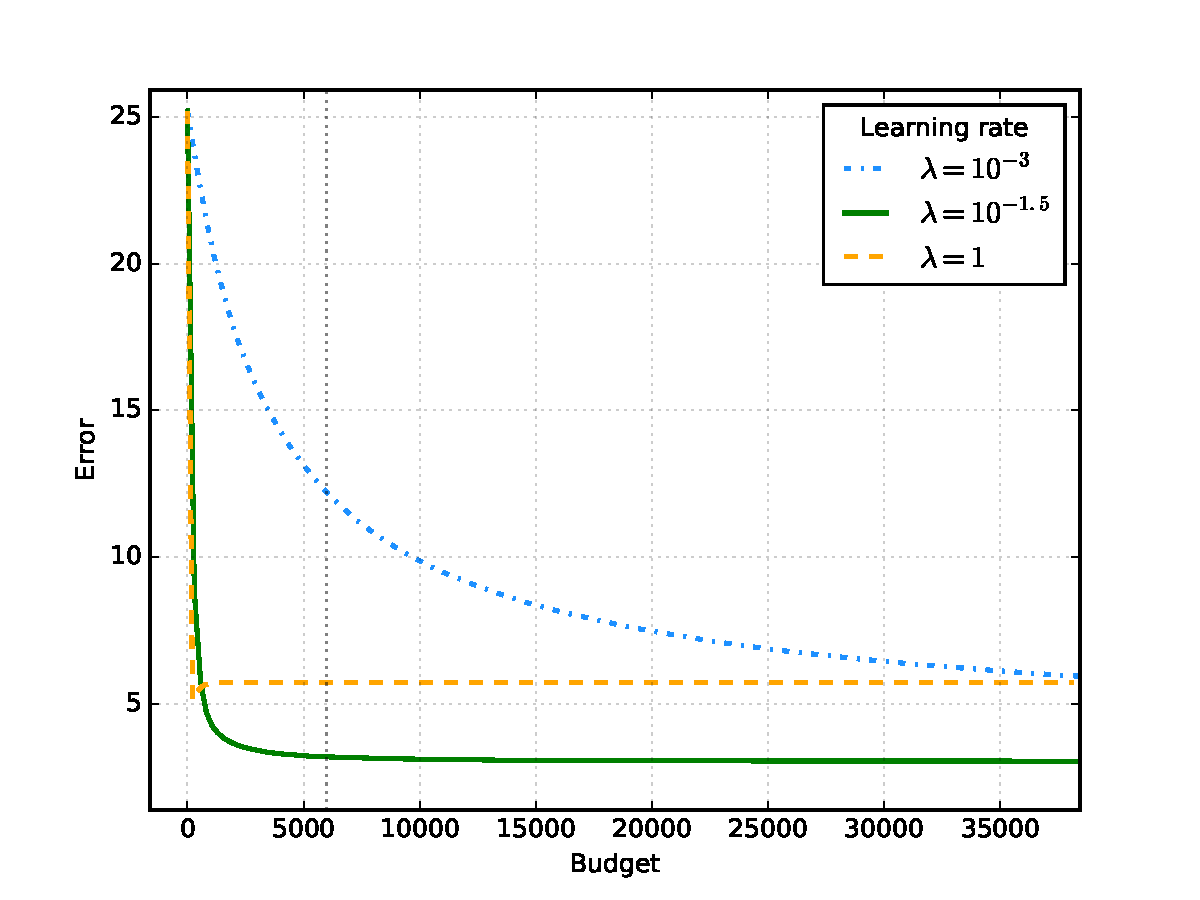
\includegraphics[width=\columnwidth]{friedman1_lr}}
%\caption{Friedman1: Testing set mean square error with respect to the budget 
%for several learning rates ($CW=\infty$,m=$\sqrt{10}$, %$T=1000$, maximum 
%%%%budget=$59900$ ($10\%$)).}
%\label{fig:learningRate}
%\end{center}
%\vskip -0.2in
%\end{figure} 

\begin{figure}[ht]
\vskip -1.2em
\begin{center}
\centerline{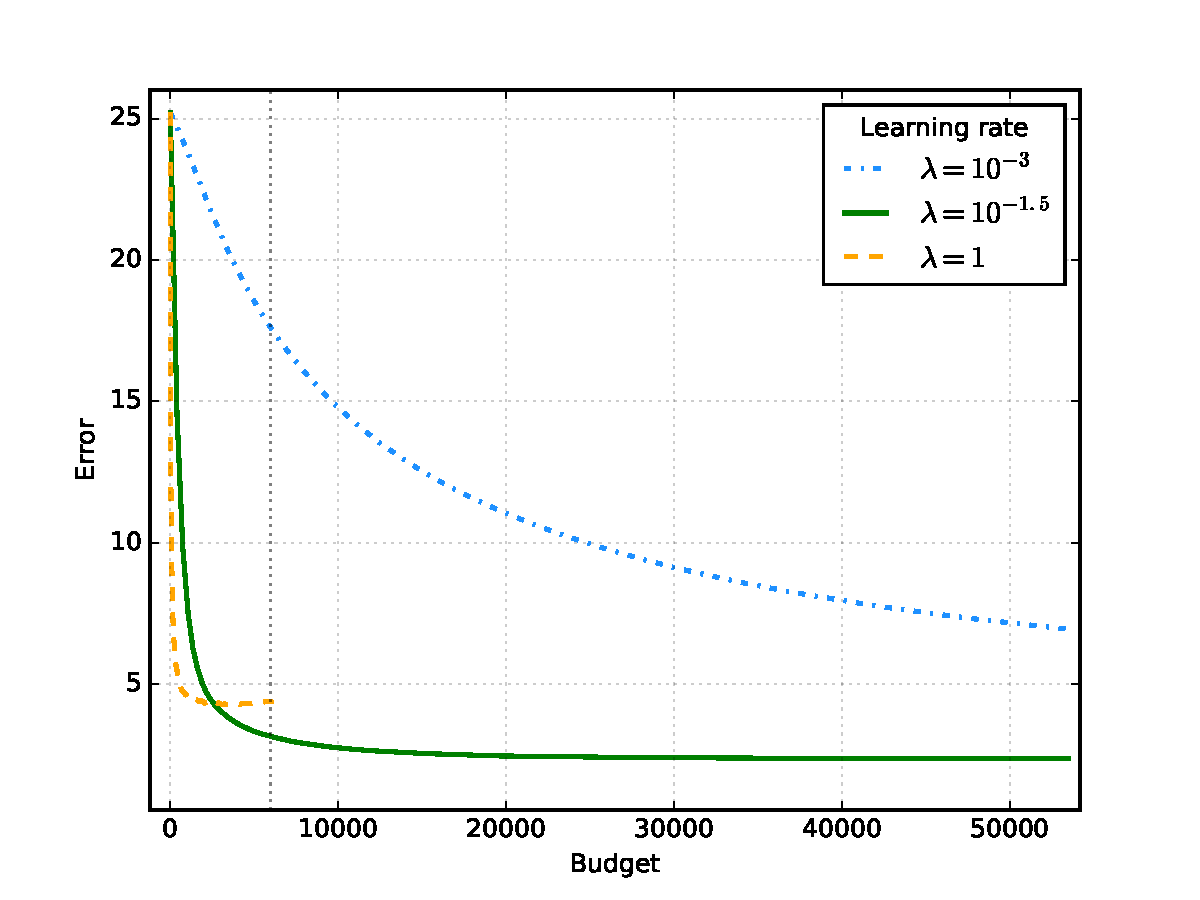
\includegraphics[width=\columnwidth]{friedman1_lr_cw1}}
\vskip -1em
\caption{Friedman1: average test set error with respect to the 
budget $B$ ($CW=1$, m=$\sqrt{10}$, $T=1000$).}
\label{fig:learningRate}
\end{center}
\vskip -0.2in
\end{figure} 

\paragraph{Learning rate.}
Figure \ref{fig:learningRate} depicts a typical evolution of the error with the 
budget for different learning rates in the case of Friedman1 (the 
budget maxes out at $59900$ nodes, corresponding to $10\%$). A unit learning 
rate will usually decrease the test set error rapidly but will then either 
saturate or overfit. 
%---not taking full advantage of the budget---or worse, overfit. 
Too small a learning rate ({\it e.g.} $10^{-3}$) will prevent the model from 
reaching its minimum in the alloted budget.  The learning rate also influences 
the forest shape, provided the candidate window size is large enough. 
Figure \ref{fig:LRShape} portrays the cumulative node distribution with respect 
to the size-ranks of the trees for $CW=\infty$, meaning that f(x) is the ratio 
of nodes of the x/T smallest trees. We can see that, for the smallest learning 
rate,  $80\%$ of the smallest trees account for approximately $43\%$ of the 
nodes. At the same stage, only $17\%$ and $13\%$ of the nodes are covered for 
the average and biggest learning rates, respectively. 


\begin{figure}[ht]
\vskip -1.2em
\begin{center}
\centerline{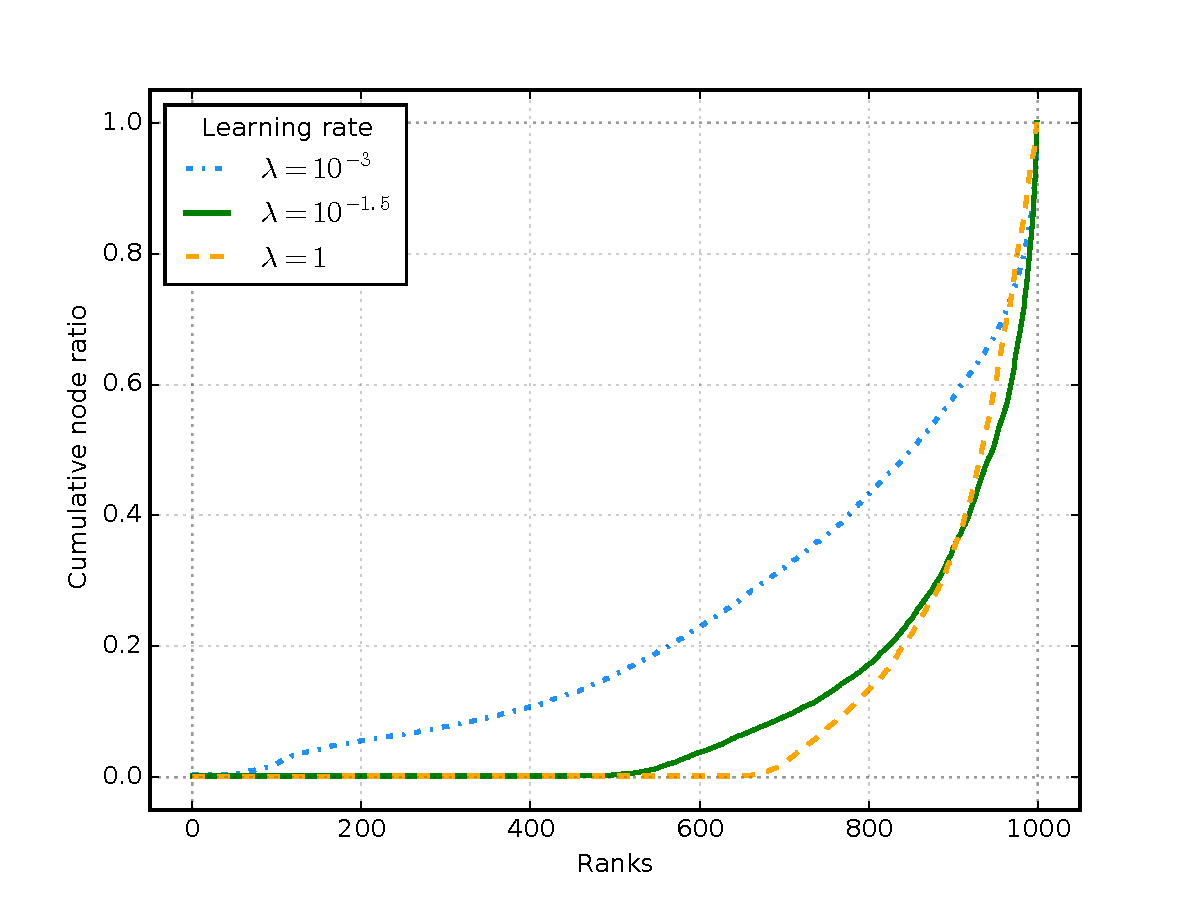
\includegraphics[width=\columnwidth]{friedman1_cumul}}
\vskip -1em
\caption{Friedman1: cumulative node distribution with respect to 
the size-ranks ($CW=\infty$, m=$\sqrt{10}$, $T=1000$, $B=10\%$).}
\label{fig:LRShape}
\end{center}
\vskip -2em
\end{figure} 

%These results are corroborated by Table \ref{tab:friedEntropy}, which holds 
%the 
%entropies of the node distribution across trees. Note that entropy has been 
%normalized so that it max out at $1$.
%
%\begin{table}[t]
%\caption{Friedman1: average normalized entropy of the node distribution across 
%trees. ($CW=\infty$, m=$\sqrt{10}$, $T=1000$, budget=$59900$ ($10\%$)).}
%\label{tab:friedEntropy}
%\vskip 0.15in
%\begin{center}
%\begin{small}
%\begin{tabular}{l|ccccccc}
%\hline
%$\lambda$ & $10^{-3}$ &  $10^{-2.5}$ & $10^{-2}$ & $10^{-1.5}$ & $10^{-1}$ & 
%$10^{-0.5}$ & 1 \\
%\hline
% & 0.94 & 0.92 & 0.90 & 0.87 & 0.85 & 0.84 & 0.84
%\end{tabular}
%\end{small}
%\end{center}
%\vskip -0.1in
%\end{table}



\begin{table}[t]
\caption{Average test set error with respect to $m$ and $\lambda$ ($CW=1$, 
$T=1000$, $B=10\%$; $\theta=3$). 
In bold is $m=\sqrt{p}$.}
\label{tab:maxFeat}
\begin{center}
\begin{footnotesize}
CT slice: mean square error
\begin{tabular}{l|ccccc}
\hline
m $\backslash$ $\lambda$  &  $10^{-2.5}$ & $10^{-2}$ & $10^{-1.5}$ & 
$10^{-1}$ & $10^{-0.5}$ \\
%\hline
%friedman
%1 & \cellcolor[gray]{0.54} 5.35 & \cellcolor[gray]{0.85} 3.35 & 
%\cellcolor[gray]{0.89} 3.05 & \cellcolor[gray]{0.87} 3.21 & 
%\cellcolor[gray]{0.78} 3.79 & \cellcolor[gray]{0.43} 6.07 \\
%{\bf 3} & \cellcolor[gray]{0.81} 3.60 & \cellcolor[gray]{0.96} 2.65 & 
%\cellcolor[gray]{1.00} 2.37 & \cellcolor[gray]{1.00} 2.39 & 
%\cellcolor[gray]{0.94} 2.75 & \cellcolor[gray]{0.68} 4.43 \\
%5 & \cellcolor[gray]{0.79} 3.76 & \cellcolor[gray]{0.92} 2.89 & 
%\cellcolor[gray]{0.97} 2.54 & \cellcolor[gray]{0.98} 2.48 & 
%\cellcolor[gray]{0.94} 2.76 & \cellcolor[gray]{0.72} 4.18 \\
%7 & \cellcolor[gray]{0.73} 4.13 & \cellcolor[gray]{0.84} 3.37 & 
%\cellcolor[gray]{0.89} 3.06 & \cellcolor[gray]{0.90} 3.03 & 
%\cellcolor[gray]{0.85} 3.34 & \cellcolor[gray]{0.63} 4.75 \\
%10 & \cellcolor[gray]{0.65} 4.63 & \cellcolor[gray]{0.74} 4.02 & 
%\cellcolor[gray]{0.77} 3.88 & \cellcolor[gray]{0.74} 4.06 & 
%\cellcolor[gray]{0.66} 4.59 & \cellcolor[gray]{0.40} 6.25 \\
\hline
{\bf 19} & \cellcolor[gray]{0.59} 27.28 & \cellcolor[gray]{0.92} 20.34 & 
\cellcolor[gray]{0.97} 19.31 & \cellcolor[gray]{0.84} 21.97 & 
\cellcolor[gray]{0.47} 29.82 \\
38 & \cellcolor[gray]{0.66} 25.78 & \cellcolor[gray]{0.96} 19.51 & 
\cellcolor[gray]{1.00} 18.63 & \cellcolor[gray]{0.89} 20.88 & 
\cellcolor[gray]{0.58} 27.62 \\
96 & \cellcolor[gray]{0.68} 25.53 & \cellcolor[gray]{0.95} 19.74 & 
\cellcolor[gray]{0.99} 18.79 & \cellcolor[gray]{0.90} 20.68 & 
\cellcolor[gray]{0.62} 26.64 \\
192 & \cellcolor[gray]{0.63} 26.55 & \cellcolor[gray]{0.89} 20.96 & 
\cellcolor[gray]{0.94} 19.92 & \cellcolor[gray]{0.86} 21.62 & 
\cellcolor[gray]{0.61} 26.87 \\
288 & \cellcolor[gray]{0.55} 28.20 & \cellcolor[gray]{0.82} 22.43 & 
\cellcolor[gray]{0.89} 20.91 & \cellcolor[gray]{0.83} 22.31 & 
\cellcolor[gray]{0.58} 27.64 \\
385 & \cellcolor[gray]{0.40} 31.42 & \cellcolor[gray]{0.70} 25.04 & 
\cellcolor[gray]{0.79} 23.11 & \cellcolor[gray]{0.74} 24.17 & 
\cellcolor[gray]{0.49} 29.56 \\
\hline
\end{tabular}
\par
Musk2: error rate ($\%$)\\
\begin{tabular}{l|ccccc}
\hline
m $\backslash$ $\lambda$  &  $10^{-2.5}$ & $10^{-2}$ & $10^{-1.5}$ & 
$10^{-1}$ & $10^{-0.5}$ \\
\hline
{\bf 12} & \cellcolor[gray]{0.40} 5.13 & \cellcolor[gray]{0.75} 3.74 & 
\cellcolor[gray]{0.90} 3.14 & \cellcolor[gray]{0.96} 2.90 & 
\cellcolor[gray]{0.97} 2.86 \\
16 & \cellcolor[gray]{0.43} 5.00 & \cellcolor[gray]{0.77} 3.67 & 
\cellcolor[gray]{0.91} 3.11 & \cellcolor[gray]{0.96} 2.91 & 
\cellcolor[gray]{0.97} 2.85 \\
41 & \cellcolor[gray]{0.56} 4.50 & \cellcolor[gray]{0.84} 3.39 & 
\cellcolor[gray]{0.94} 3.00 & \cellcolor[gray]{0.95} 2.93 & 
\cellcolor[gray]{0.96} 2.93 \\
83 & \cellcolor[gray]{0.62} 4.24 & \cellcolor[gray]{0.87} 3.26 & 
\cellcolor[gray]{0.96} 2.92 & \cellcolor[gray]{0.97} 2.88 & 
\cellcolor[gray]{0.96} 2.90 \\
124 & \cellcolor[gray]{0.66} 4.11 & \cellcolor[gray]{0.89} 3.20 & 
\cellcolor[gray]{0.96} 2.89 & \cellcolor[gray]{0.99} 2.79 & 
\cellcolor[gray]{1.00} 2.75 \\
166 & \cellcolor[gray]{0.66} 4.11 & \cellcolor[gray]{0.89} 3.19 & 
\cellcolor[gray]{0.95} 2.94 & \cellcolor[gray]{0.98} 2.84 & 
\cellcolor[gray]{0.97} 2.86 \\
\hline
\end{tabular}
\end{footnotesize}
\end{center}
\vskip -0.2in
\end{table}

\paragraph{Number of features.}
Table \ref{tab:maxFeat} shows how the error varies at $10\%$ for $CW=1$ with 
respect to both the learning rate $\lambda$ and $m$, the number of features 
examined for a split, in the case of CT slice and Musk2, two datasets with many 
features.
Interestingly, the error tends to vary continuously over those two parameters. 
%When there is more than one local minima, it is not far from the global one. 
%This makes for an easy joint optimization of those two parameters. 
On both datasets, it appears that the choice of learning rate (global 
parameter) is more critical than the number of features (local parameter). The 
optimal number of features remains problem-dependent, though. 
%Not much of a conclusion..




\begin{figure}[ht]
\begin{center}
\centerline{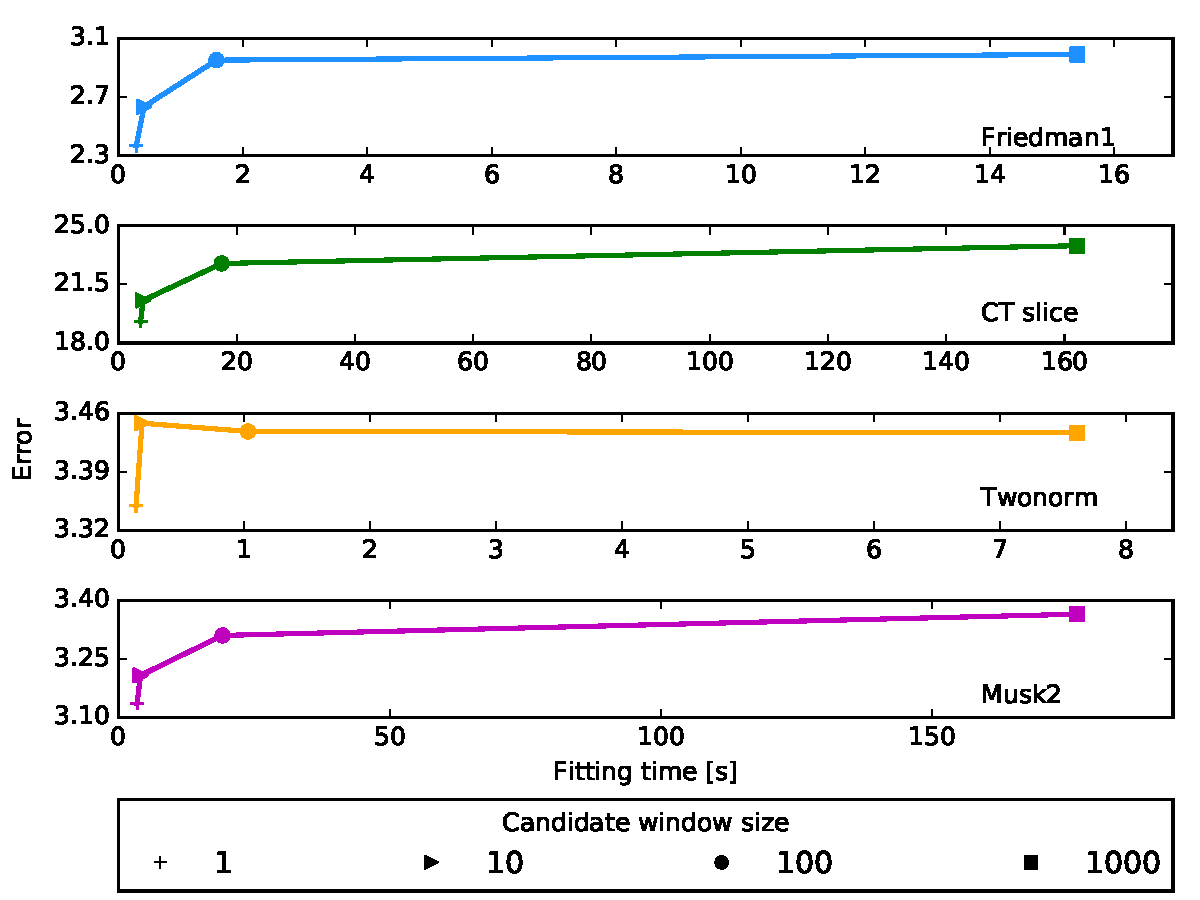
\includegraphics[width=\columnwidth]{cw_4}}
\vskip -0.8em
\caption{Average test set error (MSE for Friedman1 and CT slice, 
error rate ($\%$) for Twonorm and Musk2) and fitting time 
with respect to $CW$
($\lambda=10^{-1.5}$, $m=\sqrt{p}$, $T=1000$, $B=10\%$; $\theta=3$).}
\label{fig:cw4}
\end{center}
\vskip -2em
\end{figure} 

\paragraph{Candidate window size.}
Figure \ref{fig:cw4} illustrates the influence of the candidate window size on
both the error and the fitting time for several datasets with
$\lambda=10^{-1.5}$, $m=\sqrt{p}$, $T=1000$ and a budget=$10\%$.  Firstly, the
linear dependence of the window size on the building time is clearly
visible. More interestingly, the smaller window size ($CW=1$) performs best on
all four datasets. All in all, this seems to be a good regularization
mechanism, allowing for a dramatic decrease of computing times while ensuring
better predictions.

Although this is representative of the regression and binary classification 
problems, this is not exactly the case of multiclassification, where increasing 
$CW$ over $1$ might improve performance slightly (see Table \ref{tab:cwMulti}).

\begin{table}[t]
\caption{Error rate ($\%$) for the trimmed exponential loss 
($\theta=3$, $\lambda=10^{-1.5}$, $m=\sqrt{10}$, $T=1000$, $B=10\%$)}
%\vskip -1em
\label{tab:cwMulti}
\begin{center}
\begin{footnotesize}
\begin{sc}
\begin{tabular}{l|cc}
\hline
Dataset & CW=$1$ & CW=$10$ \\
\hline
Waveform & 14.51 $\pm$ 0.67 & \bestA 14.05 $\pm$ 0.82 \\
Vowel & 15.90 $\pm$ 1.35 & \bestA 10.87 $\pm$ 1.61 \\
Mnist & 4.05 $\pm$ 0.25 & \bestA 3.66 $\pm$ 0.31 \\
Letter & 9.07 $\pm$ 0.53 & \bestA 5.88 $\pm$ 0.32 \\
\hline
\end{tabular}
\end{sc}
\end{footnotesize}
\end{center}
\vskip -0.2in
\end{table}



\begin{table}[t]
\vskip -1em
\caption{Test set error with respect to the initial 
number of trees $T$ ($m=\sqrt{p}$, $\lambda=10^{-1.5}$, same budget $B=10\%$; 
$\theta=3$).}
\vskip -0.4em
\label{tab:poolsizeError}
\begin{center}
\begin{footnotesize}
Friedman1: mean square error\\
\begin{tabular}{c|cc}
\hline
T & CW=$1$ & CW=$\infty$ \\
\hline
10 & 7.88 $\pm$ 0.64 & 7.62 $\pm$ 0.71 \\
100 & 3.31 $\pm$ 0.41 & 3.60 $\pm$ 0.35 \\
1000 & 2.37 $\pm$ 0.24 & 3.05 $\pm$ 0.29 \\
10000 & 2.26 $\pm$ 0.20 & 3.18 $\pm$ 0.28 \\
\hline
\end{tabular}
\par
Twonorm: misclassification rate ($\%$) \\
\begin{tabular}{c|cc}
\hline
T & CW=$1$ & CW=$\infty$ \\
\hline
10 & 7.47 $\pm$ 0.73 & 7.05 $\pm$ 0.29 \\
100 & 3.44 $\pm$ 0.16 & 3.52 $\pm$ 0.13 \\
1000 & 3.35 $\pm$ 0.22 & 3.43 $\pm$ 0.23 \\
10000 & 3.53 $\pm$ 0.25 & 3.87 $\pm$ 0.32 \\
\hline
\end{tabular}
\end{footnotesize}
\end{center}
\vskip -0.2in
\end{table}


\begin{table}[t]
\caption{Friedman1: average normalized node distribution entropy with respect 
to $T$ and $\lambda$ ($m=\sqrt{p}$, same budget $B=10\%$).}
\vskip -0.4em
\label{tab:poolsizeEntropy}
\begin{center}
\begin{footnotesize}
%Friedman1\\
\begin{tabular}{c|c|ccc}
\hline
 & CW=$1$ & \multicolumn{3}{c}{CW=$\infty$} \\
T $\backslash$ $\lambda$ & * & $10^{-3}$ & $10^{-1.5}$ & $1$ \\
\hline
%10 & 100.00 & 100.00 & 100.00 & 99.93 \\
100 & 99.89 & 99.84 & 99.24 & 98.48 \\
1000 & 98.15 & 94.49 & 87.32 & 83.72 \\
10000 & 97.20 & 89.12 & 76.23 & 68.99 \\
\hline
\end{tabular}
%\par
%Twonorm \\
%\begin{tabular}{c|c|ccc}
%\hline
% & CW=$1$ & \multicolumn{3}{c}{CW=$\infty$} \\
%T $\backslash$ $\lambda$ & $10^{-1.5}$ & $10^{-3}$ & $10^{-1.5}$ & $1$ \\
%\hline
%10 & 99.85 & 99.85 & 99.88 & 99.90 \\
%100 & 99.93 & 99.92 & 99.91 & 99.93 \\
%1000 & 97.90 & 96.99 & 91.55 & 91.78 \\
%10000 & 93.31 & 87.08 & 83.48 & 79.99 \\
%\hline
%\end{tabular}
\end{footnotesize}
\end{center}
\vskip -0.2in
\end{table}

\begin{table}[t]
\caption{Friedman1: fitting time (seconds) with respect to $T$ and 
$\lambda$ ($m=\sqrt{p}$, same budget $B=10\%$).}
\vskip -0.4em
\label{tab:poolsizeTime}
\begin{center}
\begin{footnotesize}
\begin{tabular}{c|c|cc}
\hline
 & CW=$1$ & \multicolumn{2}{c}{CW=$\infty$} \\
T $\backslash$ $\lambda$ & * & $10^{-3}$ &  $1$ \\
\hline
100 & 0.34 $\pm$ 0.07 & 0.35 $\pm$ 0.07 &  0.32 $\pm$ 0.07 \\
1000 & 0.59 $\pm$ 0.12 & 3.84 $\pm$ 0.18 & 2.78 $\pm$ 0.54 \\
10000 & 1.55 $\pm$ 0.02 & 25.95 $\pm$ 1.05 & 20.69 $\pm$ 
2.92 \\
\hline
\end{tabular}
\end{footnotesize}
\end{center}
\vskip -0.2in
\end{table}

\paragraph{Number of trees.}
The initial number of trees is an intricate parameter, as it impacts model
predictions, the fitting time and the shape of the forest.

Table \ref{tab:poolsizeError} focuses on the errors with $m=\sqrt{p}$ and 
$\lambda=10^{-1.5}$. Unsurprisingly, the models perform badly when it has only 
10 trees at its disposal; this leaves only little room for the learning 
algorithm to optimize globally. The more trees is not always better, however. 
When the candidate window is infinitely large, this might be due to 
overfitting: there are so many candidates to choose from that over-optimization 
hurts the model. When the window size is $1$, this is more directly linked to 
the forest shape.

Table \ref{tab:poolsizeEntropy} holds the normalized entropy of the node
distribution across trees for Friedman1.  By ``normalized'', we mean that the
entropy was divided by its maximal possible value $\log_2 T$ and then
multiplied by $100$.  Only one value is reported for the case $CW=1$ as the
forest has always the same shape, whatever the learning rate $\lambda$. The
evolution of the entropy for a fix number of trees when $CW=\infty$ has already
been commented on (see Figure \ref{fig:LRShape}).  It is rendered more
obvious when the initial number of trees is larger, however, meaning that GIF
is able to exploit the greater freedom offered by the additional trees.  When
$CW=1$, the distribution is much closer to being uniform (entropy close to
$100$) than when the learning algorithm can adapt the forest shape.  If this
shape does not agree with the data, the model might perform less well.
Nevertheless, as we saw, $CW=1$ yields better result on all but the multiclass
problems, and $T=1000$ seems to be adequate in average. %Poor way to conclude

The number of trees also impacts the learning time, as depicted by Table 
\ref{tab:poolsizeTime}. The linear increase in computing time in the case of 
$CW=\infty$ is due to the global optimization of the chosen node that must run 
through all the candidates. In the case of $CW=1$, the computing time is 
almost not burdened by the number of trees. The slight increase is actually 
related to the forest shape: since the distribution of node tends to be more 
uniform, the algorithm must run through more examples while optimizing the 
weights (higher part of the trees).


\subsection{A preliminary comparison with Boosting}
\label{subsec:boosting}


\begin{table}[t]
\caption{Test set error (MSE/error rate ($\%$)) for stump least-sqaure 
Boosting/Adaboost under budget constraints ($\lambda=10^{-1.5}$).}
\vskip -0.2em
\label{tab:boosting}
\begin{center}
\begin{footnotesize}
\begin{sc}
\begin{tabular}{l|c|c}
\hline
Datasets & $B=10\%$ & $B=1\%$ \\
\hline
Friedman1 & 4.53 $\pm$ 0.23 & 3.86 $\pm$ 0.10 \\
Abalone & 5.17 $\pm$ 0.20 & 4.83 $\pm$ 0.20 \\
CT slice & 82.44 $\pm$ 3.80 & 68.73 $\pm$ 1.92 \\
Hwang $\times 10{-2}$ & 97.88 $\pm$ 2.33 &  88.62 $\pm$ 1.73 \\
\hline
Ringnorm & 5.48 $\pm$ 0.55 & 6.71 $\pm$ 0.99 \\
Twonorm & 5.09 $\pm$ 0.56 & 5.98 $\pm$ 0.47 \\
Hastie & 5.65 $\pm$ 0.34 & 7.10 $\pm$ 0.41 \\
Musk2 & 2.70 $\pm$ 0.37 & 4.20 $\pm$ 0.28 \\
Madelon & 11.30 $\pm$ 0.68 & 11.33 $\pm$ 0.69 \\
\hline
\end{tabular}
\end{sc}
\end{footnotesize}
\end{center}
\vskip -0.2in
\end{table}


%Although not our starting point, Boosting is another method to build ensemble 
%of trees. In this section, we compare how GIF fares against it. 

In this section, we carry out a first comparison of GIF with Boosting. To
submit Boosting to the budget constraint, we have used stumps as base learners
and have made as many trees as were necessary to meet the constraint.  We have
used the same learning rate as for GIF in Table \ref{tab:reg}. Regression has
been tackled with least square Boosting \cite{hastie2009} and classification
with Adaboost \cite{adaboost}, so that the same losses are used for GIF and
Boosting. Scikit-Learn was used as Boosting implementation.

Table \ref{tab:boosting} holds the errors for Boosting at $1\%$ and $10\%$. In
the default setting, GIF beats Boosting on all regression datasets except
Abalone where it performs slightly less well. Interestingly, Boosting also
overfits on Abalone and Hwang. The situation is more contrasted in
classification, where Boosting outperforms GIF on Hastie and Musk2 for both
budget constraints. Notice that stumps are not optimal for Hwang and CT slice,
where a depth of $2$ would yield lower errors of $11.09 \pm 0.25$ and $8.40 \pm
0.19$ at $10\%$ and $1\%$ respectively for Hwang and $33.53 \pm 1.65$ and
$36.67 \pm 1.36$ at $10\%$ and $1\%$ respectively for CT slice. However, this
does not change the conclusions regarding the comparison with GIF.

GIF (with $CW=1$) is faster in both learning and prediction than Boosting, as
confirmed in Table \ref{tab:boostingTime}. Firstly, Boosting's base learners
are traditional decision trees, which are slower to fit than ET for a given
structure. Secondly, Boosting's base learners are shallow and they can thus take
less advantage of the partitioning induced by the trees.

Overall, the performances of Boosting and GIF in terms of errors are somewhat 
similar. Sometimes GIF's extra-layers of regularization, combined with a 
greater variety of depths pays off and sometimes not. However, GIF is faster in 
both learning and prediction.


\begin{table}[t]
\caption{Musk2: fitting/prediction times (seconds). Stump Adaboost versus GIF  
(trimmed loss with $\theta=3$, $T=1000$, $m=\sqrt{p}$, $CW=1$) for $B=10\%$ and 
$\lambda=10^{-1.5}$.}
\vskip -0.2em
\label{tab:boostingTime}
\begin{center}
\begin{footnotesize}
\begin{tabular}{l|c|c}
\hline
& Adaboost & GIF \\
\hline
Fitting & 399.17 $\pm$ 60.91 & 1.53 $\pm$ 0.04 \\
Prediction & 28.39 $\pm$ 5.43 & 0.31 $\pm$ 0.07 \\
\hline
\end{tabular}
\end{footnotesize}
\end{center}
\vskip -0.2in
\end{table}



%\subsection{Comparison with post-pruning}

\section{Conclusion and perspectives}
\label{sec:conclusion}

In this paper, we introduced the Globally Induced Forest (GIF) whose goal is to
produce lightweight yet accurate tree-based ensemble models by sequentially
adding nodes to the model. Contrary to most tree-aware
techniques, our method is framed as a pre-pruning method that does not require
the {\it a priori} building of the whole forest. Several hyper-parameters
govern the learning algorithm. We have proposed a set of default parameters
which seems to work quite well in average, beating the baselines, under mild
and severe memory constraints. Needless to say that the setting of these
parameters can be further optimized if necessary, although this goes against
the philosophy of building directly the pruned forest. Of the most interest is
the conclusion that it is usually better not to optimize the choice of
nodes. In other words, letting the algorithm optimize the forest shape
is---surprisingly---harmful. Although it complicates the choice of the initial
number of trees, this makes the algorithm extremely fast.

%% Although motivated as a pre-pruning technique for decision forests, the
%% resulting algorithm shares similar traits with Boosting, the main differences
%% being the extra layers of regularization and the forest shape adaptability. Note
%% that adapting the forest shape with Boosting has been explored by
%% \citet{johnson2014regforest}, with a different goal in mind.

The main focus of subsequent works should be to handle multiclass problems
better. %% Aside from
%% that, frequent uses of the tree-based techniques, such as measuring feature
%% importances and using them as codebook, should be examined.
Several extensions can also be thought of. For instance, one could consider
introducing both children at the same time at each iteration or allow for the
refitting of the already chosen nodes by leaving them in the candidate
list. Finally, we would also like to explore further the comparison between GIF
and boosting methods, in particular \citet{johnson2014regforest}'s regularized
greedy forests, which share similar traits with GIF.

%% The split might also be optimized globally if the candidate window is
%% small enough, although this might result in overfitting. Multi-output losses
%% which take into account the correlation between the outputs can also be
%% proposed.  Finally, it would be interesting to investigate close variants, such
%% as introducing both children at the same time or designing an online algorithm
%% for when an extremely lightweight model is desired on a very large dataset.

\section*{Acknowledgements} 
Part of this research has been carried out while Arnaud Joly was a research 
fellow of the FNRS, Belgium. Computational resources have been provided by the 
Consortium des \'Equipements de Calcul Intensif (C\'ECI), funded by the Fonds 
de la Recherche Scientifique de Belgique (F.R.S.-FNRS) under Grant No. 
2.5020.11. This work is also supported by the DYSCO IUAP network of the Belgian 
Science Policy Office.


\bibliography{gif}
\bibliographystyle{icml2017}

\end{document} 
